\documentclass{sigchi}

% Use this section to set the ACM copyright statement (e.g. for
% preprints).  Consult the conference website for the camera-ready
% copyright statement.

% Copyright
\CopyrightYear{2016}
%\setcopyright{acmcopyright}
\setcopyright{acmlicensed}
%\setcopyright{rightsretained}
%\setcopyright{usgov}
%\setcopyright{usgovmixed}
%\setcopyright{cagov}
%\setcopyright{cagovmixed}
% DOI
\doi{http://dx.doi.org/10.475/123_4}
% ISBN
\isbn{123-4567-24-567/08/06}
%Conference
\conferenceinfo{L@S 2017,}{April 20--21, 2017, Cambridge, MA, USA}
%Price
\acmPrice{\$15.00}

% Use this command to override the default ACM copyright statement
% (e.g. for preprints).  Consult the conference website for the
% camera-ready copyright statement.

%% HOW TO OVERRIDE THE DEFAULT COPYRIGHT STRIP --
%% Please note you need to make sure the copy for your specific
%% license is used here!
% \toappear{
% Permission to make digital or hard copies of all or part of this work
% for personal or classroom use is granted without fee provided that
% copies are not made or distributed for profit or commercial advantage
% and that copies bear this notice and the full citation on the first
% page. Copyrights for components of this work owned by others than ACM
% must be honored. Abstracting with credit is permitted. To copy
% otherwise, or republish, to post on servers or to redistribute to
% lists, requires prior specific permission and/or a fee. Request
% permissions from \href{mailto:Permissions@acm.org}{Permissions@acm.org}. \\
% \emph{CHI '16},  May 07--12, 2016, San Jose, CA, USA \\
% ACM xxx-x-xxxx-xxxx-x/xx/xx\ldots \$15.00 \\
% DOI: \url{http://dx.doi.org/xx.xxxx/xxxxxxx.xxxxxxx}
% }

% Arabic page numbers for submission.  Remove this line to eliminate
% page numbers for the camera ready copy
% \pagenumbering{arabic}

% Load basic packages
\usepackage{balance}       % to better equalize the last page
\usepackage{graphics}      % for EPS, load graphicx instead 
\usepackage[T1]{fontenc}   % for umlauts and other diaeresis
\usepackage{txfonts}
\usepackage{mathptmx}
\usepackage[pdflang={en-US},pdftex]{hyperref}
\usepackage{color}
\usepackage{booktabs}
\usepackage{textcomp}

% Some optional stuff you might like/need.
\usepackage{microtype}        % Improved Tracking and Kerning
% \usepackage[all]{hypcap}    % Fixes bug in hyperref caption linking
\usepackage{ccicons}          % Cite your images correctly!
% \usepackage[utf8]{inputenc} % for a UTF8 editor only

% If you want to use todo notes, marginpars etc. during creation of
% your draft document, you have to enable the "chi_draft" option for
% the document class. To do this, change the very first line to:
% "\documentclass[chi_draft]{sigchi}". You can then place todo notes
% by using the "\todo{...}"  command. Make sure to disable the draft
% option again before submitting your final document.
\usepackage{todonotes}
\usepackage{bbding}
\usepackage{enumitem}
\usepackage{makecell}
\usepackage{multirow}
\usepackage{subfigure,graphicx}
\usepackage[group-separator={,}]{siunitx}
\usepackage{minted}
%avoid widow and orphan lines
\widowpenalty10000 
\clubpenalty10000

\newmintedfile[javacode]{java}{
fontfamily=tt,
fontsize=\tiny,
linenos=true,
numberblanklines=true,
numbersep=10pt,
numbersep=5pt,
gobble=0,
frame=leftline,
framerule=0.4pt,
framesep=2mm,
funcnamehighlighting=false,
tabsize=4,
obeytabs=false,
mathescape=false
samepage=false, %with this setting you can force the list to appear on the same page
showspaces=false,
showtabs =false,
texcl=false
}
% Paper metadata (use plain text, for PDF inclusion and later
% re-using, if desired).  Use \emtpyauthor when submitting for review
% so you remain anonymous.
\def\plaintitle{1. \\
2.}
\def\plainauthor{First Author, Second Author, Third Author,
  Fourth Author}
\def\emptyauthor{}
\def\plainkeywords{Individual differences, Java, MOOC, Student modeling}
\def\plaingeneralterms{Documentation, Standardization}

% llt: Define a global style for URLs, rather that the default one
\makeatletter
\def\url@leostyle{%
  \@ifundefined{selectfont}{
    \def\UrlFont{\sf}
  }{
    \def\UrlFont{\small\bf\ttfamily}
  }}
\makeatother
\urlstyle{leo}

% To make various LaTeX processors do the right thing with page size.
\def\pprw{8.5in}
\def\pprh{11in}
\special{papersize=\pprw,\pprh}
\setlength{\paperwidth}{\pprw}
\setlength{\paperheight}{\pprh}
\setlength{\pdfpagewidth}{\pprw}
\setlength{\pdfpageheight}{\pprh}

% Make sure hyperref comes last of your loaded packages, to give it a
% fighting chance of not being over-written, since its job is to
% redefine many LaTeX commands.
\definecolor{linkColor}{RGB}{6,125,233}
\hypersetup{%
  pdftitle={\plaintitle},
% Use \plainauthor for final version.
  pdfauthor={\plainauthor},
%  pdfauthor={\emptyauthor},
  pdfkeywords={\plainkeywords},
  pdfdisplaydoctitle=true, % For Accessibility
  bookmarksnumbered,
  pdfstartview={FitH},
  colorlinks,
  citecolor=black,
  filecolor=black,
  linkcolor=black,
  urlcolor=linkColor,
  breaklinks=true,
  hypertexnames=false
}

% create a shortcut to typeset table headings
% \newcommand\tabhead[1]{\small\textbf{#1}}

% End of preamble. Here it comes the document.
\begin{document}

\title{
%1. In Search of Student Stereotypes: Mining  Problem-Solving Behavior in a Programming MOOC\\
Mining Student Coding Behaviors in a Programming MOOC: There Are No Actionable Learner Stereotypes}

\numberofauthors{4}
\author{%
  \alignauthor{Author 1, Author 2\\
    \affaddr{Affiliation 1}\\
    \affaddr{City 1, Country 1}\\
    \email{e-mail addresses 1,2}}\\
  \alignauthor{Author 3\\
    \affaddr{Affiliation 3}\\
    \affaddr{City 3, Country 3}\\
    \email{e-mail address 3}}\\
  \alignauthor{Author 4\\
    \affaddr{Affiliation 4}\\
    \affaddr{City 4, Country 4}\\
    \email{e-mail address 4}}\\
}

\maketitle

\begin{abstract}
It is natural to think about students and their abilities in broad categories. In literature, there are frequent references to \textit{weaker} students, \textit{fast learners}, \textit{struggling} students, etc. Teachers in classrooms and computer-based systems are often framing their interaction with the student based on these stereotypes. However, are these stereotypes real?\\
In this paper, we are reviewing a few simpler readily available student grouping factors like gender or education level together and a number of innovative approaches to cluster students based on their \textit{genomes} of problem-solving behaviors. Each of the approaches to form student cohorts is validated by comparing models of student learning: do students in different groups, in fact, learn differently. After considering ten approaches to grouping students taking a traditional programming course and a programming MOOC, we conclude that there are no two distinct student stereotypes that can be actionable in a group-based     adaptation setting.
\end{abstract}

\category{D.2.3}{Software Engineering}{Coding Tools and Techniques}[Object-oriented programming]
%\category{D.2.6}{Software Engineering}{Programming Environments}[Interactive environments]
%\category{K.3.1}{Computers And Education}{Computer Uses in Education} [Computer-assisted instruction (CAI), Computer-managed instruction (CMI)]
%\category{K.3.2}{Computers And Education}{Computer and Information Science Education} [Computer science education, Self-assessment]

\keywords{\plainkeywords}

\section{Introduction}

The problem of student performance in MOOCs has been a topic of extensive research over the last three years. It has been observed that student performance in a MOOC could vary considerably with many students solving only a fraction of problems or dropping from the MOOC completely \cite{breslow2013studying}. Consequently, considerable research also focused on explaining and predicting student performance in MOOC. It has been argued that the ability to predict performance could help to identify a cohort of weaker students sufficiently early to help them in succeeding a MOOC. Early attempts to identify weak and strong students focused mostly on examining various demographic features such as gender, level of education, or country of origin as a source for performance prediction \cite{breslow2013studying}. These attempts brought little success, on the contrary, a significant number of both strong and weak students were found within each demographic category. The more recent research attempted to identify cohorts of strong and weak students by examining student course behavior through MOOC log mining. This research focused mostly on coarse-grain traces of student access to various parts of MOOC such as videos, questions, or discussion forums. While many attempts focused on behavior mining brought interesting results \cite{wen2014identifying, toth2014discovering,wang2015investigating}, the results of different studies were to some extent contradictory. In some cases more diligent access to course content was a positive sign of good performance \cite{sharma2015identifying}. In other cases, it was negatively correlated with success \cite{champaign2014correlating}, or skipping content was a good sign \cite{guo2014demographic}. It has been argued that patterns of student access to course content are, to a considerable extent, influenced by the starting level of knowledge rather than by differences in student approaches to learning.

In this paper, we present our attempt to separate strong and weak learners by using a very different kind of behavior analysis. First, we focused on problem-solving behavior, which, we hoped, is less affected by the starting knowledge and more related to student individual learning approach than content access behavior. Second, we examined student behavior in a more finer-grain level tracing individual steps to solve each problem rather than registering all that as one content-level access. Finally, before moving to group elicitation and clustering, we ensured that we found reliable and repeatable patterns of behavior for every student. The result of our behavior mining attempt was, however, unexpected. While we were able to discover groups of students that considerably differ by their problem-solving behavior patterns, these groups were not the expected stereotypical ``weak'' and ``strong'' students and were useless for stereotype-based performance prediction. Instead, the differences between groups represented different problem-solving styles that have some correlation with performance, but, as our data demonstrated, does not define it. 

The rest of the paper is structured as follows. In the next section, we offer a brief review of similar work including MOOC behavior mining and analysis of assessment data in programming. Next, in two separate sections, we introduce our dataset and the performance prediction approach that we use to assess our ability to distill performance-based stereotypes. To demonstrate some simple application of this approach, we start by confirming the absence of demography-based stereotypes. Following that, we present our sequence-based behavior mining approach and its application to our dataset to discover patterns of student problem-solving behavior. Next, we present and discuss the results of behavior-based clustering. We conclude with a general discussion of lessons learned. 

\section{Related Work}

\subsection{Student Behavior Analysis in MOOCs}

Due to a large volume of available data and a surprisingly low completion rate, the analysis of student behavior in MOOCs emerged as an important topic just a few years ago. Perhaps one of the very first studies on MOOC and behavior was the work in \cite{breslow2013studying} that focused on the amount of time that students spent in various activities, as well on demographic information about the students. In a more recent attempt \cite{anderson2014engaging}, a taxonomy of individual learner behaviors was developed to examine the different behavior patterns of high- and low-achieving students. Another attempt was the work in \cite{wang2015investigating} that adopted a content analysis approach to analyze students' cognitively relevant behaviors in a MOOC discussion forum and explored the relationship between the quantity and quality of that participation with their learning gains. In a similar attempt, \cite{sharma2015identifying} presented a hierarchy to categorize MOOC student based on their styles into different engagement groups.

Overall, past studies focused mostly on resource usages such as viewing course lectures, quizzes, assignments, and discussion forum activities to find the behavior of different groups of student and relate the behaviors with high- and low- learning. However, there is some evidence from past work that demonstrates that focusing solely on resource usage might not lead to a reliable approach to separate weak and strong students \cite{champaign2014correlating}. %For example, \cite{champaign2014correlating} showed that the use of the resource is not a good indicator for success as they found that work on the resource and improvement of skill were negatively correlated. %Additionally, \cite{bergner2015methodological} showed that there are methodological challenges inherent in analyzing activity data to find behavior and relating them to performance measures such as the grade.
Unlike the past studies, the current work analyzes student behaviors by finding micro-patterns in student problem-solving activities rather than by examining resource usage. Two similarly-minded attempts can be found in \cite{toth2014discovering} that focused on the search for problem-solving strategies, and \cite{wen2014identifying} that defined study habits by mining student topic-based navigation. None of these attempts explored behaviors by getting deep into how student solves problems, though. %\cite{wen2014identifying} mined navigation sequences that were obtained from student browsing of course materials, or \cite{toth2014discovering} used surface-level features of problem-solving behavior to cluster students by their problem-solving behavior.

\subsection {Assessment Data Analysis in Programming}
Analyzing student solutions to programming problems (assignments) has started to receive much attention during the past years. %One main reason for the growing interest is the increased availability and large-scale application of tools that automatically assess students programs submitted as problem solutions. %This great functionality enabled instructors to rise the number of programming assignments in the course while offering students multiple submission attempts for each assignment \cite{douce2005automatic} and real-time feedback for each submitted solution.  
%As a result, more and more submission data is accumulated over different programming courses creating an opportunity for researchers to understand how student write their program and also identify programming behaviors common to the groups of students. 
Recent work used submission data to reveal multiple correct and incorrect ways to solve the same problem \cite{huang2013syntactic,glassman2015overcode}, build an intelligent scaffolding system \cite{rivers2013automatic}, model student's knowledge in a program development context \cite{piech2012modeling,yudelson2014investigating}, predict student  %success \cite{Ahadi:2015} or 
grade \cite{murphy2009retina}, and understand student coding behavior %by compilations attempts \cite{blikstein2011using} or
by conceptual analysis of the program code \cite{Hosseini2014Psychology}.

The current paper contributes to the existing body of literature on analysis of assessment data by using compilation and submission data collected from students' problem solving activities in a Java MOOC to understand (1) individual patterns of problem-solving (coding) behavior, (2) impact of the discovered behaviors on students performance in the programming course, and (3) implications of the behaviors for accurately modeling student knowledge. 
%\subsection{Data-driven student performance prediction}
%\todo[inline]{@Michael}
%\textcolor{green}{Folks, since we are running our of space and time, we might as well to skip this section. Prediction approach is not innovation or contribution; it is simply a way to check where we are, i.e., evaluation approach. It would be sufficient to add a few words about  this and other approaches when we introduce it.}
%\textcolor{red}{Recent work on modeling student knowledge from programming submissions: \cite{yudelson2014investigating}}
%%%%%%%
\section{Data}

The data for the study comes from a total of four introductory programming courses, and MOOCs organized at a research-oriented University in Europe during 2014 and 2015. A single iteration of the programming course lasted seven weeks, was taught in Java. %, and used a blended online textbook that covered variables, basic I/O, methods, conditionals, loops, lists, arrays, elementary search algorithms and elementary objects. %The main focus of the course is learning to program, and thus, programming is practiced a lot. 
Each week, students worked on tens of programming assignments with varying complexity. Less complex assignments were given when a new topic or construct (e.g., loops) was introduced, and as students created a number of smaller programs with those constructs, they moved to larger assignments that required use of multiple constructs. The students worked on the assignments in NetBeans environment. %an integrated development environment called  which is an external free application and not a part of the online textbook. 
The assignments were downloaded into the programming environment with the Test My Code-plugin \cite{testMyCode}, which was used to assess the students' code automatically, and to collect data from the programming process of those students who consent to the use of their data for research purposes. 

The collected data included key-presses with time, assignment information, and student id, and was aggregated to describe meaningful events in the students' programming process. The events used for this study were \emph{running the program}, \emph{running the tests for the program}, and \emph{submitting the program for grading}; also, the first five generic events (inserting or removing text) were included for each assignment to make it possible to analyze the transitions to the meaningful events. For each event, information on program compilation and correctness were extracted for the data in a posthoc analysis using JUnit test sets, and finally, \emph{programming concepts} for each problem-solving state were extracted using JavaParser~\cite{hosseini2013javaparser}.

In addition to the data gathering from the programming process, students were given a demographic questionnaire that surveyed the students' age, gender, programming background and the highest level of education attained so far. From the total of 2739 distinct students that started the courses, 1788 were included in the initial sample (the cutoff was 2500 recorded events which correspond to roughly a $33^{rd}$ percentile of the first week of the course workload). Out of those, 798 students answered the questionnaire and were included in the final analysis sample. Table~\ref{tab:participantstatistics} shows key statistics for all participants.%, and the highest level of attained education for the participants. 


\begin{table*}[thb]
  \centering
  \begin{tabular}{l r r r r r r r r r r r r}

    &   \multicolumn{2}{c}{\small{Student sample}} & 
        \multicolumn{1}{c}{\small{Age}} & 
        \multicolumn{1}{c}{\small{Gender}} & 
        \multicolumn{1}{c}{\small{Programming background}} & 
        \multicolumn{1}{c}{\small{Prior education}}\\
        
        {\small\textit{Course}} & 
        {\small \textit{Initial}} & 
        {\small \textit{Final}} & 
        {\small \textit{min / mean / max}} & 
        \multicolumn{1}{c}{\small \textit{M / F / NA}} & 
        {\small \textit{None / Some / More }} & 
        {\small \textit{Pri.\&Sec. / College / Grad }}\\
    \midrule
    MOOC 2014 & 1286 & 90 & 16 / 32.3 / 65 & 90\% / 9\% / 1\% & 4\% / 81\% / 15\% & 63\% / 12\% / 25\%\\
    Traditional 2014 & 263  & 192 & 18 / 23.2 / 44 & 62\% / 38\% / 0\% & 59\% / 38\% / 3\%  & 78\% / 3\%  / 19\% \\
    MOOC 2015 & 984  & 372 & 15 / 30.8 / 66 & 77\% / 22\% / 1\% & 30\% / 60\% / 10\%  & 58\% / 13\% / 29\%\\
    Traditional 2015 & 206 & 144 & 19 / 24.3 / 45 & 63\% / 35\% / 2\% & 56\% / 39\% / 5\% & 74\% / 3\%  / 23\% \\
    % \bottomrule
  \end{tabular}
  \caption{Background information on the students that took the courses.}~\label{tab:participantstatistics}\vspace{-16pt}
\end{table*}

% students who reported background details _and_ were included through the filtering
% k2014-mooc    90
% k2015-ohjelmointi    372
% s2014-ohpe    192
% s2015-ohpe    144 

% TODO: discuss this more.

% \textcolor{red}{Del.Peter also suggests removing} While the number of participants may seem low to those accustomed to the MOOC participant numbers reported in the literature, the context in which this study was conducted is limited in the number of possible participants due to the language of the course. When including all those speaking a language as their primary or secondary language, a course with 1,000 participants in the language of the course would correspond to a course with 250,000 participants in a course organized in English. 

% \textcolor{red}{Del. Peter also suggests removing} Although no socioeconomic factors were available for this study, the studied population is relatively homogenous, and the educational system in the context is inclusive. That is, all universities and colleges are state funded, and there are no tuition fees. Moreover, students can receive benefits such as direct funding from the state, assuming that they progress in their degree work. Even in such a context, there is still need and interest for courses open for all.

% TODO: ..notes on why the dataset is not publicly available; at this point, the dataset is not publicly available, as data at such granularity can be directly used to infer the students who have been typing~\cite{Longi:2015}.

\section{The Assessment Approach}

In this work, we are trying to determine whether separating students into various cohorts for the group-based adaptation is useful. In particular, we are interested whether we could find such distinct groups of students that their members learn differently (such as stereotypically ``good'' and ``bad'' students). As a criteria to judge whether we were able to obtain the desired ``adaptation-level'' split between groups when looking at multiple ways to group students, we use differences between models of student learning in each group. Our rule of thumb is that if groups are truly different in how their members learn, the group models would be different regarding performance. 

Before turning to the innovative approaches to separate students by their programming behavior, we demonstrate our evaluation approach by assessing simpler ways of grouping them. These simpler groupings would include those known apriori (e.g., demographics, prior achievements) and those known aposteriori (e.g., overall course performance). By comparing innovative approaches to the simpler ones, we also monitor whether our behavior-based approach is different enough. Naturally, we would prefer behavior clustering results that do not align with simpler groupings. After evaluating simpler approaches to student grouping, we will cover student clustering using programming behavior mining. All approaches will be validated using groups/clusters models of learning and predicting across group/cluster boundaries. %\textcolor{red}{Student modeling values will also be compared.}

\section{Using Models of Student Learning for Grouping/Cluster Validation}

\subsection{Modeling Student Learning}

Before discussing validation of student groupings/clusters, we would like to describe our  student modeling approach. For modeling student knowledge acquisition, we considered models based on logistic regression. In particular, we used a model called Performance Factors Analysis \cite{pfa2009}. This model represents student abilities as a random factor $\theta_i$, concept difficulties as fixed-factor intercepts $\beta_k$, skill learning rates from correct and incorrect submissions as $\gamma_k$ and $\rho_k$ respectively. Equation~(\ref{eq:pfa}) shows the canonical form of the PFA. Here, $s_{ik}$ and $f_{ik}$ are the numbers of prior attempts at a concept that were successful and failed respectively. \vspace{-14pt}

\begin{equation}
    \Pr(Y_i = 1 | \theta, \beta, \gamma, \rho) = inv.logit~( \theta_i + \sum_{k}{(\gamma_k s_{ik} + \rho_k f_{ik})}~
    \label{eq:pfa}
\end{equation}\vspace{-14pt}

Our choice of a model was based on the compensatory nature of the PFA -- multiple concepts used in student's submissions, together, form a cumulative signal that results in a successful or an unsuccessful outcome. The other candidate modeling approach -- Bayesian Knowledge Tracing (BKT) \cite{bkt1995} -- is not intended for the cases when multiple concepts are associated with student transactions since it violates independence assumptions of the Hidden Markov Model that BKT is using.

We have made two modifications to the PFA both of which improved the overall model fit. First, we have switched from globally defined concepts for all problems to within-problem concepts. Indeed, a for-loop concept crucial for one problem could be irrelevant for another. Second, we used each concept's usage count within the problem code toward the opportunity count and $log1p$-transformed opportunity counts after that. Both of these modifications proved useful in the work by Yudelson et al. \cite{yudelson2014investigating} that considered the data from the same source, but different academic years. These modifications only changed the definitions of what is a concept and how the success and failure attempts are accumulated. The canonical form of PFA remained the same.

In contrast to \cite{yudelson2014investigating}, we pre-processed the data differently. First, every snapshot of the student code was treated as an atomic unit of data. It was deemed successful if all tests passed, otherwise the problem attempt was unsuccessful. Second, we only considered snapshots that students were testing, running, or submitting their code -- i.e., purposefully testing it for correctness. Intermediate snapshots were not considered for student modeling. If a student tested, ran, and then submitted the code without modifications in between, it was regarded as one attempt. Third, we considered all concepts that were used in student's code. Only considering changes in concepts with or without special treatment for removals (as in \cite{yudelson2014investigating}) lead to model performance degradation under our data pre-processing setup. Finally, we considered only students for whom we had background information (798 out of 1788 students).

Due to our modifications, the number of PFA concept parameters went from 143*3-1 = 428 to 143*240*3-1 = 102,959. However, because of the problem-concept matrix sparsity, the actual number of parameters was 13542*3-1 = 40,625. Also, given the size of the data containing about 392,000 student submissions, it was not possible to use conventional statistical packages. We used a modified LIBLINEAR tool \cite{liblinear2008}. The modification\footnote {\url{https://github.com/IEDMS/liblinear-mixed-models}} was in the form of an additional solver that allowed grouped $L^2$-penalties to approximate random factors. The modified LIBLINEAR retained the ability of the original version to tackle large datasets successfully.


\subsection{Validating By Cluster Models' Cross-Prediction}

The primary goal of this work is to find at least two groups of students in our sample that \textit{learn differently}. Following the approach piloted in \cite{yudelson2014bdbbd}, given the breakdown of a student sample into $n$ groups/clusters, we sub-sample each group 20 times to extract 80 students as a training set and 20 students as a test set. Sub-sample models are built from each of the 80-student training set. We then use each of the $n*20$ models to predict three corresponding sub-samples: one sample is matching the group the model was built on, the rest are from the other group(s). Finally, we plot $n^2$ model accuracies (means and standard errors) $n$ of which represent model performance within the group and the rest are between the groups.

Our criterion for students in different groups \textit{learning differently} is that within-group model performance would be significantly better than between-group model performance. In the case where $n>2$, that should be true for at least two groups out of $n$. An example of the \textit{ideal} separation is shown in Figure~\ref{fig:graph-predict} in red. Here, a model built on group $A$ is superior to the model built on group B when predicting test data from group $A$. At the same time, when predicting test data of group $B$, model $B$ wins on \textit{its own ground}. Thus, groups $A$ and $B$ are sufficiently different that their respective models, when cross-predicting, do not perform well outside of their source student sub-sample. An \textit{expected} case is marked in blue. This situation was repeatedly found by authors of \cite{yudelson2014bdbbd}. In this case, there is a domination of one model over the others, irrespective of what sub-sample the test data is drawn from. Such cases are marked in blue (model $B$ vs. model $C$). Finally, a \textit{sub-optimal} case of model $A$ vs. model $C$ (marked in green) is when one model wins on \textit{its own ground} (here, $A$) but does not have the edge over or loses to the other model (here, $C$).

\begin{figure}[thb]
\centering
   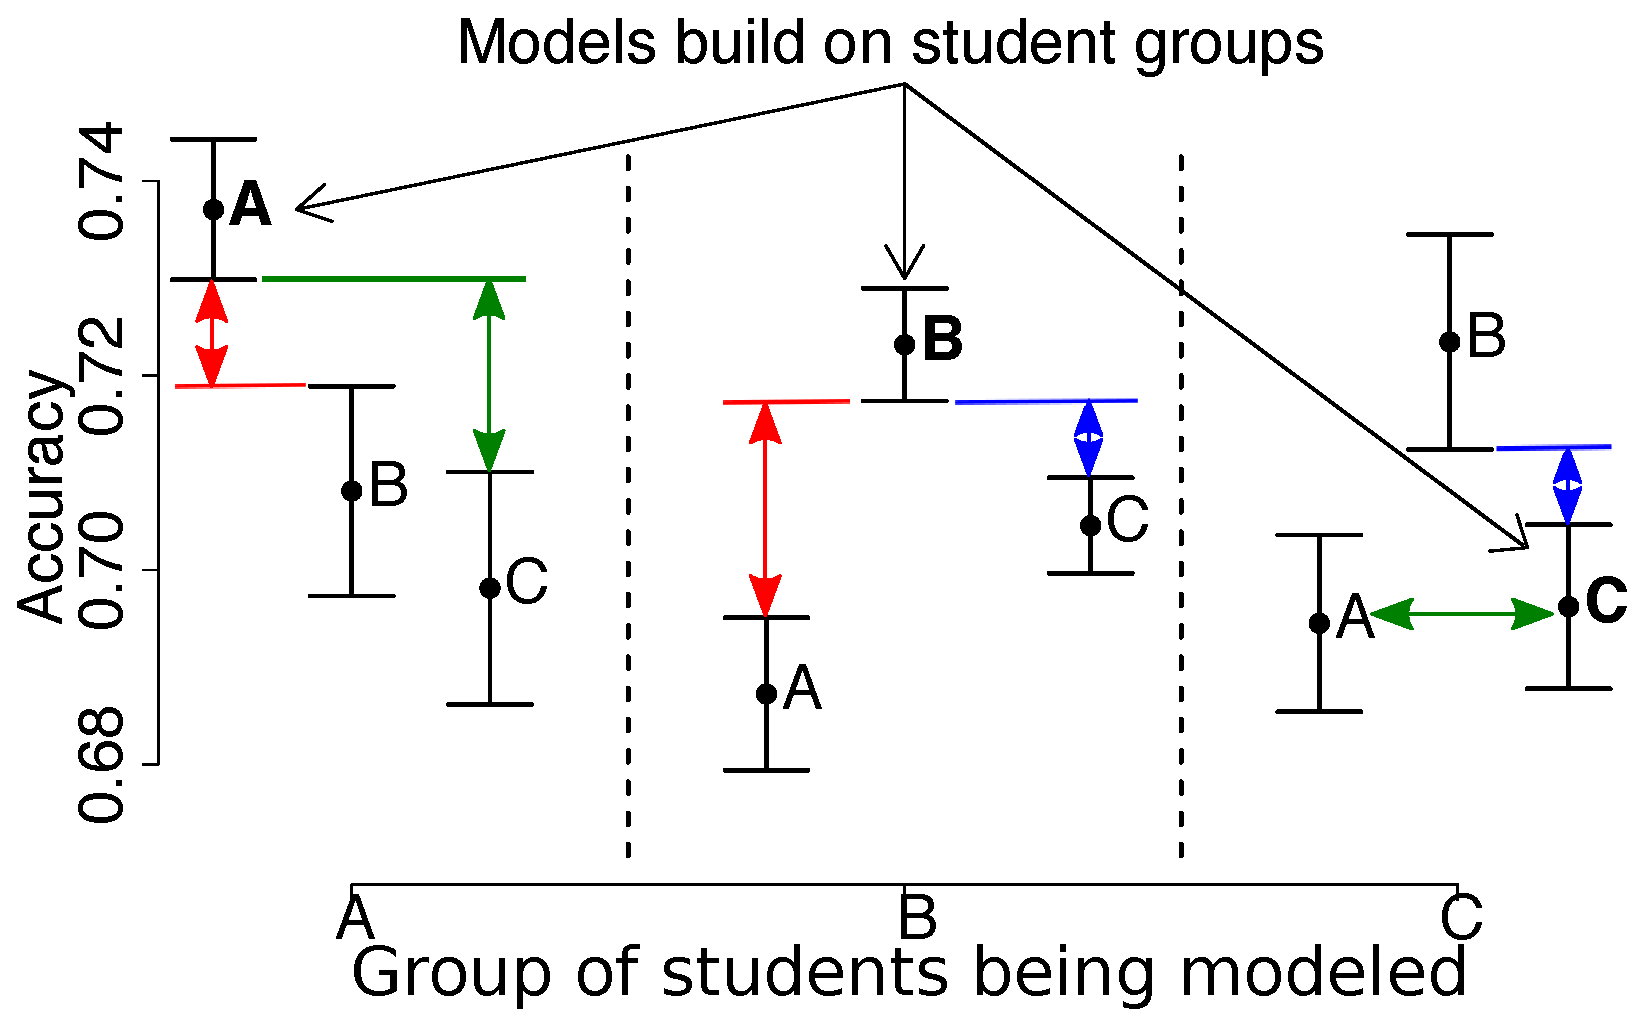
\includegraphics[width=0.75\columnwidth]{figures/cross-predict_examples.eps}
\caption{Between-group student model prediction accuracy differences (means and standard errors). Red arrows mark an \textit{ideal} case, blue -- \textit{expected} case, green -- \textit{sub-optimal} case.}%\vspace{-13pt}
\label{fig:graph-predict}
\end{figure}

\section{Simple Student Grouping}

As an example of an application of our assessment approach, we first examine simpler demographic- and course performance-based approaches to student grouping. This data are readily available to us in the form of background information collected during the course or represent overall course statistics available at the end. These groupings are summarized in the top five rows of Table ~\ref{table:behavior-groups}.

\begin{table*}[h]
\centering
\begin{tabular}{ll|cccc|ccccc|cc}
         &               & \multicolumn{9}{c|}{\small{Group/cluster label overlaps}} & \multicolumn{2}{c}{\small{Prediction diff.}} \\
\cmidrule{3-13}
\small{Approach} & \small\textit{Cluster sizes}  & \small\textit{Edu.} & \textit{\small{\#Trans.}} & \textit{\small{P.Solv.}} & \textit{\small{\%Corr.}} & \textit{\small{B1}}     & \textit{\small{B2}}     & \textit{\small{B3}}     & \textit{\small{B4}}    & \textit{\small{B5}}    & \textit{\small{Score}} & \begin{tabular}[c]{@{}l@{}}\textit{\small{Cluster}}\\ \textit{\small{to note}}\end{tabular}\\
\midrule
\small\textit{Gender$\dagger$}   & {570, \textbf{228}}  & 0.36 & 0.03 & 0.06 & 0.07 & 0.10   & 0.02   & 0.13   & 0.18  & 0.19  & 0.33  & F. \\
\small\textit{Edu.$\ddagger$}    & {524, 154, 120} & & 0.04 & 0.12 & 0.06 & 0.18   & 0.15   & 0.12   & 0.24  & 0.12  & 0.00   &  \\
\small\textit{\#Trans.$\ddagger$} & {266, 266, \textbf{266}} & & & 0.40 & 0.30 & 0.18   & 0.21   & 0.34   & 0.21  & 0.24  & 0.67  & Hi \\
\small\textit{P.Solv.$\ddagger$}  & {218, 316, 264} & & & & 0.09 & 0.15   & 0.18   & 0.31   & 0.09  & 0.04  & 0.00  & \\
\small\textit{\%Corr.$\ddagger$}  & {266, 266, 266} & & & & & 0.22   & 0.18   & 0.12   & 0.28  & 0.28  & 0.00  &  \\
\midrule
\small\textit{B1}       & {\textbf{383}, 415}      & & & & &        & 0.58   & 0.43   & 0.58  & 0.51  & 0.67  & 1 \\
\small\textit{B2}       & {\textbf{416}, 382}     & & & & &        &        & 0.70   & 0.44  & 0.51  & 0.67  & 1 \\
\small\textit{B3}       & {258, \textbf{158}, 382} & & & & &        &        &        & 0.40  & 0.51  & 0.67  & 2 \\
\small\textit{B4}       & {\textbf{295}, 503}     & & & &  &        &        &        &       & 0.69  & 0.67  & 1 \\
\small\textit{B5}       & {389, \textbf{272}, 137} & & & & &        &        &        &       &       & 0.67  & 2 \\ 
\bottomrule
\multicolumn{13}{l}{\footnotesize $\dagger$ Male and Female; $\ddagger$ These groupings have 3 levels: Low, Medium, and High}
\end{tabular}
\caption{Validating approaches to clustering students.}\vspace{-10pt}
\label{table:behavior-groups}
\end{table*}

\textbf{Gender}. The majority of students were males (about 71\%).

\textbf{Education level} was split into three groups. There were 524 students that had Primary and Secondary Education, 154 students went to college, and 120 students were in grad school.

\textbf{Number of transactions}. Students were split into three equal percentile groups -- low, medium, and high -- by the total number of problem attempts. Authors of \cite{yudelson2014bdbbd} that employed a similar approach to investigating student groupings, reported that a subset of students that yielded more data (and covered more material) yielded a globally superior model as well. This grouping is to serve as our check for that phenomenon. 

\textbf{Problems Solved} is an agglomerative Euclidean-distance clustering result over four course-level count variables: problems solved (at least one submission 100\% correct), partially solved (at least one submission >0\%correct), attempted but not solved (at least one submission of 0\% correct), and not attempted. This clustering yielded three groups of students: low (mostly not attempting problems), high (mostly solving problems), and medium (everyone else). This grouping is to serve as an overall student performance measure.

\textbf{Percent Correct} is a split with three percentile groups with low, medium, and high values of overall percent correct of the times students purposefully tested, ran, or submitted their code. This grouping is to separate students by diligence.

\subsection{Validating Simple Groupings}

Top left quadrant of the ``Group/cluster label overlaps'' columns in Table~\ref{table:behavior-groups} contains pairwise similarities of five simple groupings. The similarities are computed as the largest overlap between the breakdowns of the students into the clusters over the total of 798 students. The overlaps are scaled to assume values from 0 to 1. There is no general threshold that we are aware of to be comparing these similarities against. We used $\leq 0.40$ as an ad-hoc rule of thumb. Thus, all pairwise overlaps of simple groupings are small enough to be noteworthy.

Our preference for the cross-prediction group separation is in the order they are listed above: \textit{ideal}, \textit{expected}, and \textit{suboptimal}. For simplicity, we score group and cluster separations. A score of $1.0$ would mean the separation is \textit{ideal}, a score of $0.67$ -- that the separation is \textit{expected}, a score of $0.33$ -- if the separation is \textit{suboptimal}, otherwise -- a score of $0.00$. Cross-prediction differences between simpler groupings are addressed in the top five rows of the ``Prediction diff.'' columns of Table~\ref{table:behavior-groups}. Out of five approaches, only two have a non-zero score. In the case of gender contrasts, a model of female students has the edge over the model of males when predicting test data of females. When predicting test data of males, both models perform the same. Concerning the total number of student transactions grouping, we see that the model of a cluster with students contributing the most data has an edge. It is better than others no matter what test data is predicted. 

\section{Behavior Mining for Clustering Students}

The key idea of our behavior mining approach is to characterize student problem-solving behavior on the level of micro-patterns that define how the student progresses to the correct solution through several incorrect solutions and how his or her knowledge grows from assignment to assignment. To build the micro-patterns, we started by processing student intermediate programming steps classifying the programming behavior at each step (Part A). Then, we applied sequential pattern mining to extract sequential micro-patterns (Part B). Next, the most frequent micro-patterns were used to build a profile vector (we call it a genome) that represented student problem-solving behavior. The stability of the behavior vector built from micro-patterns was checked to ensure the validity of our approach to mining problem-solving behaviors (Part C). Each of these parts is explained in detail as follows.


\subsection{Part A. Processing Intermediate Programming Steps}

To determine student problem-solving behavior, we started by looking into how students progressed in coding their problem solutions. We utilized intermediate programming steps, namely snapshots, that were captured from student coding activities. Each snapshot recorded the submitted code and its correctness on a suite of tests designed for each problem.

Figure \ref{fig:snapshotAB} illustrates two consecutive snapshots of a student for the problem named ``Bigger Number''. This problem asks a student to write a program that receives as input two numbers from a user and then prints out the larger of the two. The student's program is analyzed via three tests that verified that the output was right when the first number was smaller than the second (Test 1), the output was right when the second number was smaller than the first (Test 2), and the student did not print anything unnecessary (Test 3). In this example, the student first wrote a program (Figure \ref{fig:snapshotA}) that passed Test 1 Test 2 when the first number was smaller than the second or vice versa. However, it did not pass Test 3 because it printed additional information when the second number was smaller than the first. After receiving this feedback, the student expanded the code by adding the ``else if'' statement (Figure \ref{fig:snapshotB}). Then the program also passed Test 3 because it did not print any unnecessary outputs when the numbers differed.

\begin{figure}[thb]
\centering
\subfigure[]{%
   \begin{minipage}[t]{0.9\linewidth}
        \javacode{codes/BiggerNumberSnapshotA.java}
   \end{minipage}
\label{fig:snapshotA}}
\quad
\subfigure[]{%
   \begin{minipage}[t]{0.9\linewidth}
        \javacode{codes/BiggerNumberSnapshotB.java}
    \end{minipage}
\label{fig:snapshotB}}
%
\caption{\textit{Bigger Number} program: (a) 1$^{st}$ snapshot, (b) 2$^{nd}$ snapshot.}%\vspace{-20pt}
\label{fig:snapshotAB}
\end{figure}

As in \cite{Hosseini2014Psychology}, to mine programming behavior, we first examine conceptual differences between consecutive snapshots -- i.e., observe which concepts were added or removed on each step, and inspect how these changes were associated with improving or decreasing the correctness of the program. We measured conceptual differences between two snapshots as the difference between their concept counts. The procedure for mining the behaviors includes two main steps: (a) labeling sequence of students' snapshots in each problem, and (b) mining micro-patterns of frequent behaviors (we call it genes), by conducting sequence mining on all of the labeled snapshots.

To label the sequence of student's snapshots in a problem, the snapshots that were captured for the student in that problem (including generic, test, run, and submit snapshots) were collected and ordered by time. Each snapshot in the sequence was labeled based on the change in the \textit{programming concepts} and \textit{correctness} from the previous snapshot. The previous snapshot for the first snapshot in the sequence was defined as snapshot $\emptyset$ where the code has no concepts and passes no tests.  Table \ref{table:labels} lists the labels that we used during labeling snapshots. \vspace{-5pt}

\begin{table}[thb]
\centering
\begin{tabular}{cccc}
 & \multicolumn{3}{c}{\small{Concepts}} \\ \cmidrule{2-4} 
\small{Correctness} & \small\textit{Increase} & \small\textit{Decrease} & \small\textit{Same} \\ \midrule
\small\textit{Increase} & a & b & c \\
\small\textit{Same} & d & e & f \\
\small\textit{Decrease} & g & h & i \\
\small\textit{Zero} & j & k & l \\ 
\end{tabular}
\caption{Labels for encoding programming behavior in a snapshot.}\vspace{-5pt}
\label{table:labels}
\end{table}

For example, to label the first snapshot in Figure \ref{fig:snapshotA}, we compare its number of concepts and correctness to the snapshot $\emptyset$ that has zero concepts and correctness. In this snapshot, student increased concepts and ratio of passed tests increased to 0.67 (passing two out of three tests). Thus, the first snapshot would be labeled as ``a''. The label for the second snapshot in Figure \ref{fig:snapshotB} would be ``a'' too because student added one more concept (``if else'') and increased the ratio of passed test to 1 (passing all the three tests). Since student had only two snapshots for the Bigger Number problem, the sequence of her snapshots would be labeled as ``{\_}aa{\_}'' -- obtained by concatenating the labels of each individual snapshot. The``{\_}'' symbol is used to show starting and ending points of sequence. 

Additionally, to distinguish between a short and long step (that is an important aspect of problem-solving behavior), another dimension could be added to each label to convey the extent of time that was spent on a snapshot. Since different students might have different speed in programming, it is reasonable to use individualized thresholds for classifying the time spent on a step as short or long. This way, a snapshot is labeled as short or long depending on the time being shorter or greater than the median of time distribution for each student. In our coding, lowercase letters (a--l) represent \textit{short} steps and uppercase letters (A--L) represent \textit{long} steps. For example, assuming that the median of time distribution for student in Figure \ref{fig:snapshotAB} is 10 minutes, and that the student spent 15 minutes to develop the code in the first snapshot and another 2 minutes to make the minor change in the second snapshot, then the sequence of her snapshots would be labeled as ``{\_}Aa{\_}''.

In total, we labeled \num{137504} sequences of snapshots that were obtained from attempts of 1788 students in 241 problems. The length of sequences ranged from 1 to 475 with the average of 5.3; \num{92549} sequences had more than one step, \num{64328} had more than two steps, \num{48195} had more than three steps, and \num{38768} had more than four steps.

\subsection{Part B. Mining Problem-Solving Micro-Patterns}
We mined frequent sequential patterns in students problem-solving sequences using the implementation of the SPAM algorithm \cite{ayres2002sequential} offered by the SPMF Library \cite{fournier2016spmf}. The input data to the SPAM consisted of 9254 sequences with at least two steps in them. SPAM discovers all frequent sequential patterns that occur in more than \textit{minsup} of students' sequences. In this work, we chose a small \textit{minsup} (e.g.,  1\% and 5\%) to capture the patterns that are less frequent and may occur only in small groups of students. Also, no gap was allowed in SPAM to force the discovered patterns to have steps that appear consecutively in students' sequences. Finally, the length of the patterns was limited to two or more as we were interested in observing how students progressed in their code in consecutive steps. 

SPAM discovered 245 frequent programming patterns occurring in more than 1\% of students sequences that were labeled with respect to change of concept, correctness, and time spent on an snapshot\footnote{Assuming that all sequences have an average length of 5, the maximum number of patterns that could be found has an order of magnitude of 8: There are $24^5$ possible sequences that could be obtained from 24 labels (a--l, A--L), and the number of possible substrings in a 5-character sequence is $5\times(5+1)/2=15$. Thus, the total number of patterns that could be found from sequences with length 5 is $24^5\times15=\num{119439360}$.}. The top 20 common patterns and their frequency of occurrence is provided in Table \ref{table:patterns}.
\begin{table}[thb]
\centering
\begin{tabular}{@{}ccc|ccc@{}}
\small\textit{Rank} & \small\textit{Pattern} & \small\textit{Frequency} & \small\textit{Rank} & \small\textit{Pattern} & \small\textit{Frequency} \\ \midrule
1 & AA & 19.78\% & 11 & Ac & 6.24\% \\
2 & AD & 13.75\% & 12 & DA & 6.22\% \\
3 & \_AA & 12.17\% & 13 & \_AD & 6.18\% \\
4 & Aa & 9.75\% & 14 & Dd & 6.15\% \\
5 & AA\_ & 8.69\% & 15 & JA & 6.13\% \\
6 & DD & 8.53\% & 16 & Jc & 6.04\% \\
7 & aA & 8.31\% & 17 & \_Af & 6.01\% \\
8 & Ad & 8.26\% & 18 & dD & 5.61\% \\
9 & Af & 8.15\% & 19 & DE & 5.57\% \\
10 & JJ & 7.22\% & 20 & Jj & 5.45\% \\ 
\end{tabular}
\caption{Top 20 frequent programming patterns occurring in more than 1\% of students' problem solving sequences.}
\label{table:patterns}
\end{table}

\subsection{Part C. Using Micro-Patterns to Represent Behavior}

We used the micro-patterns discovered by sequential pattern mining to build individual behavior profiles as frequency vectors that showed how frequently each micro-pattern from a discovered set of 245 appeared in the given student's problem-solving behavior. The frequency vectors were normalized so that the frequency of micro-patterns in each vector added up to 1. This approach has been first introduced in \cite{guerra2014problem} where it was used to find problem-solving behaviors in parameterized exercises. Following this paper, we also call the micro-pattern-based student profile as the \textit{problem-solving genome}.

To ensure that the vector of micro-patterns frequencies can capture stable characteristics of the student (i.e., is it as stable as a real genome), \cite{guerra2014problem} suggested to check the stability of the vector by splitting student sequences into two ``halves'' and build her/his behavior vector from each of the two halves. If the two half-vectors (i.e., profiles build separately from each half of split data) of the same student were closer to each other than to half-vectors of other students, then we have strong evidence to claim that the behavior profile vector (genome) is stable. Following this suggestion, we split student sequences in two ways: once by randomizing sequences and dividing them into halves (random-split), and once by ordering sequences by time and dividing them into early and late halves (temporal-split). Then, we built behavior vectors for each half and calculated pairwise distances between the first and second half-vector of the student (self-distance), and first/second half-vector of the student with first/second half-vectors of other students (others-distance). The distance between half-vectors was calculated using Jensen-Shannon (JS) as it is a common measure used for computing distance between frequency distributions.

A paired Wilcoxon signed rank test was performed to compare self-distance and others-distance. For the random-split, self-distance $(Mean=0.3485,SE=0.0025)$ was found to be significantly lower than others-distance $(Mean=0.6586,SE=0.0010)$, $p<0.0001$. Similar results were obtained with the temporal-split, while the self-distance in the temporally split half-vectors $(Mean=0.4249,SE=0.0022)$ was larger than randomly split half-vectors, it was still significantly smaller than the others-distance $(Mean=0.6534,SE=0.0010)$, $p < .0001$. These observations supported stability of using micro-pattern frequencies to represent student's problem-solving behavior. Moreover, the behavior profiles obtained with the proposed approach could uniquely characterize student problem-solving behavior and distinguish the student from others.

Once we established stable vector-based profiles of student behavior, our next step is to use micro-pattern representation of problem-solving behavior to group students based on their problem-solving styles. The next section explains behavior groups that we found and their impact on student performance.

\section{Building and Examining Behavior-based Groups}

\subsection{Clustering Students into Similar Behavior Groups}

To identify similar problem-solving behavior groups, we built behavior vector of micro-patterns frequencies for each student and clustered students by using these vectors. To build the behavior vector, we used problem-solving sequences of each student obtained from all problems that they attempted during the course. Each sequence represented consecutive snapshots that were captured while students were developing the program as a solution for a problem. We tried five different settings for clustering students behavior (see Table \ref{table:clsetting}), changing the clustering method (Hierarchical, Spectral), and number of clusters (2,3). The last four settings labeled the snapshots based on concepts, correctness, and time student spent on the snapshot, while the first setting did not consider time. Also, the number of micro-patterns used in the labeling process differed, 45 patterns that were used in building behavior vectors in the first setting, were obtained by setting SPAM \textit{minsup} to 5\%. The number of patterns in the rest of the settings was 245, those setting were obtained by setting SPAM \textit{minsup} to 1\%.

\begin{table}[thb]
\centering
%\small\addtolength{\tabcolsep}{0pt}
\begin{tabular}{rrclcc}
\small\textit{No.} & \small\textit{\#Patterns} & \small\textit{Minsup} & \small\textit{Clustering Method} & \small\textit{\#Clusters} & \small\textit{Time}\\ \midrule
1 & 45 & 5\% & Hierarchical & 2 & \\
2 & 245 & 1\% & Hierarchical & 2 &  \small{\Checkmark} \\
3 & 245 & 1\% & Hierarchical & 3  & \small{\Checkmark} \\
4 & 245 & 1\% & Spectral & 2 & \small{\Checkmark} \\
5 & 245 & 1\% & Spectral & 3 & \small{\Checkmark} \\ 
\end{tabular}
\caption{Settings of the frequent programming pattern clustering.}%\vspace{-5pt}
\label{table:clsetting}
\end{table}
 
\subsection{Interpreting Discovered Clusters}

In this section, we examine in more details the nature of behavior-based grouping. To make the differences clearer, we use settings with two clusters. As the clustering similarity and our manual analysis demonstrated, all three two-cluster settings separated students into two similar groups, one group with more constructive building steps and one group who often massaged the code (i.e., added/reduced concepts without increasing the code correctness), and/or struggled in consecutive steps with no success. The settings with three clusters yielded a similar grouping for students as well, except that it separated a third group who had mixed behaviors, being closer to other two clusters in a subset of micro-patterns. As an example, Figure~\ref{fig:clusters} illustrates the behavior group that we obtained by Spectral clustering with two clusters (see Table~\ref{table:clsetting}, row 4). The Y-axis shows the frequencies of the top-20 micro-patterns for the two clusters. These patterns are re-ordered by the absolute difference between the two cluster.

\begin{figure*}[thb]
  \centering
  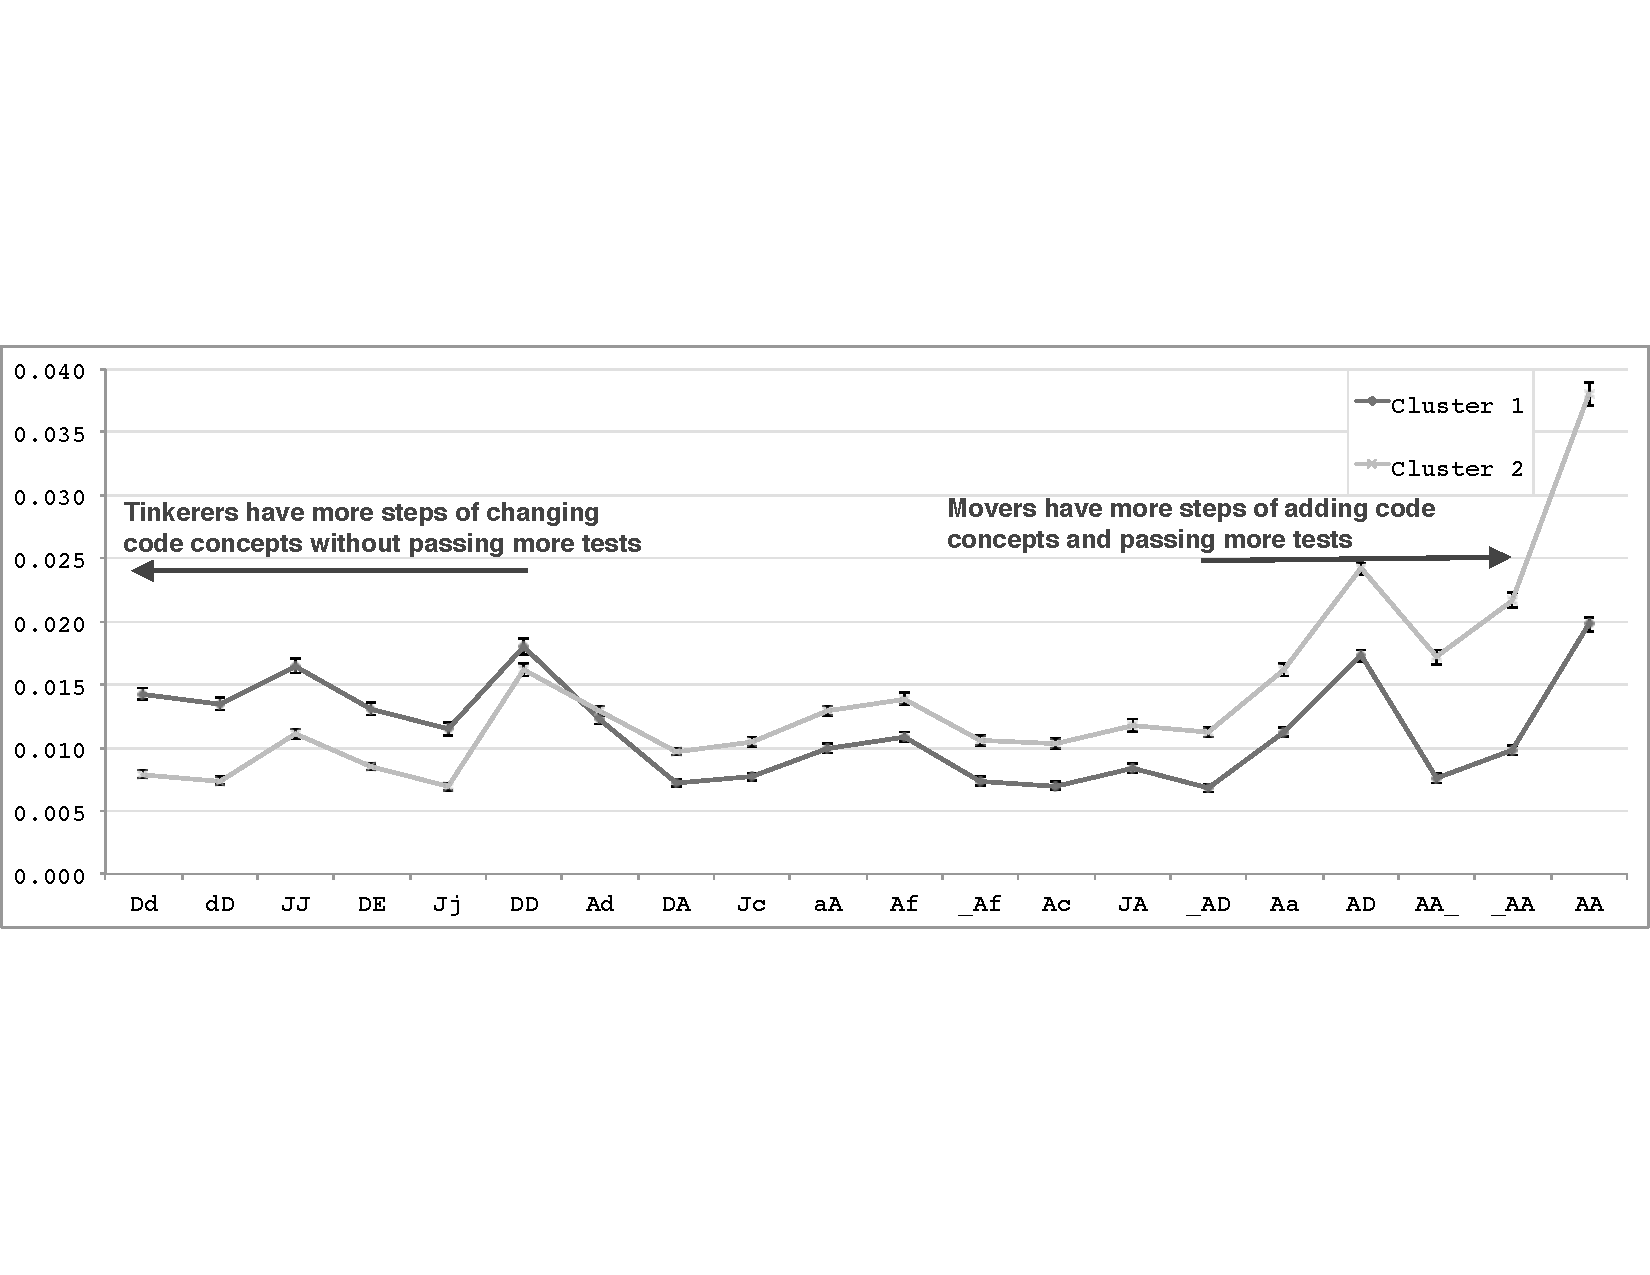
\includegraphics[width=15cm]{figures/Cluster_SpecPrevSnapAdaptTime2Sup1.pdf} %for two clusters
  \caption{Top 20 programming patterns and their ratio of occurrence in each cluster. Patterns are ordered by absolute difference of ratios between Cluster 1 (tinkerers) and Cluster 2 (movers), and error bars represents standard error of the mean.}~\label{fig:clusters} \vspace{-10pt}
\end{figure*}

As the figure shows, the groups differ by the frequency of micro-patterns on the extreme sides of the plot. As the left side shows, students in cluster 1 have higher frequency ``tinkering'' patterns (\textit{Dd}, \textit{dD}, \textit{JJ}, \textit{DE}, \textit{Jj}) while the right side shows that the students in cluster 2 demonstrate much higher frequency of careful building patterns (\textit{Aa}, \textit{AD}, \textit{AA{\_}}, \textit{{\_}AA}, \textit{AA}). More specifically, students in cluster 1 frequently increased the conceptual content of their programs in consecutive steps with long time spent on at least one of those steps (\textit{Dd}, \textit{dD}), spending long time for increasing concepts in one steps and then taking another long step decreasing concepts of their program (\textit{DE}), or they spent a long time at least on one step to increase the program concept but not only failed in increasing the correctness but jumped back to the point that no test was passed (\textit{JJ},  \textit{Jj}). On the other hand, students in cluster 2 do considerably less ``tinkering'' while focusing on large incremental building steps at which they often spent a long time on building their program. They often have long steps in which they added more concepts to the code and successfully increased its correctness or, at least did not degrade code correctness (\textit{AD}). They have these building steps, more frequently, when they started developing their program (\textit{\_AA}), while they were on mid-stages of code development (\textit{AA}, \textit{Aa}, \textit{AD}), and also at the time they ended development (\textit{AA\_}).

Our manual examination of clusters hinted that the behavior-based split separated students not by their performance, but rather by their preferred problem-solving approach. In fact, these two groups can be mapped to what Perkins et al. (1986) called \textit{tinkerers} and \textit{movers} \cite{perkins1986conditions}. Movers gradually add concepts to the solution while increasing the correctness of the solution in each step. On the other hand, tinkerers try to solve a programming problem by writing some code and then making changes in the hopes of getting it to work. 

\section{Validating Behavior-Based Clusters}

\subsection{Overlaps Between Clustering Approaches} 

Values in the top right quadrant of the ``Groups/cluster label overlaps'' rows in Table \ref{table:behavior-groups} (rows that show overlaps with simplified groupings) are all $\leq 0.40$ (below our ad-hoc threshold). This means that none of the five behavior-based clustering results align with demographics, background, or overall course performance. This is the proof that behavior-based clusters are orthogonal to simpler ways to group students and we consider that as a positive validation. Overlaps between behavior-based clustering results are all above $0.40$, highest when 2 and 3 cluster versions of the same approach are compared ($0.70$ for B2 vs. B3 and $0.69$ for B4 vs. B5). However, as clustering approaches B1 to B5 could be thought of as a sequence of incremental improvements, higher overlaps are expected.

\subsection{Validating Behavior-based Clusters by Cross-Prediction}

Bottom five rows under the header ``Prediction diff.'' in Table~\ref{table:behavior-groups} describe between-cluster model prediction differences, both the scores and the noteworthy clusters. None of the behavioral clustering approaches were scored as \textit{ideal}. Namely, we have not found at least two clusters that were voted as sufficiently different by the cluster models of student learning. All of the clustering approaches, however, received an \textit{expected} score: there was one cluster in each approach that dominated over at least over one other cluster model-wise.

To graphically illustrate some of these results, refer to Figure~\ref{fig:graph-clusters-B1}, where accuracies of cluster models cross-prediction are shown for Behavior-based clustering B1. There, we see that cluster 1 model wins when predicting test data from both clusters. Figure~\ref{fig:graph-clusters-B5} is an illustration for cross-prediction accuracy differences in the case of Behavior-based clustering B5. Cluster 2, here, has superior prediction accuracy over cluster 1 in all test data bins, so does cluster 3.

\begin{figure}[thb]
\centering
   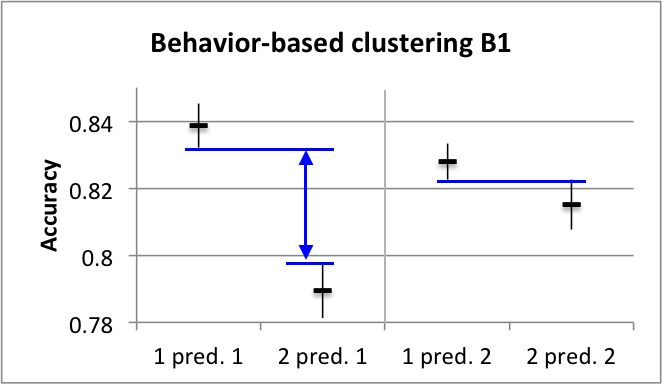
\includegraphics[width=0.7\columnwidth]{figures/behavior_clust_B1.png}
\caption{Between-cluster student group model prediction accuracy differences for Behavior-based clustering B1.}\vspace{-5pt}
\label{fig:graph-clusters-B1}
\end{figure}

\begin{figure}[thb]
\centering
   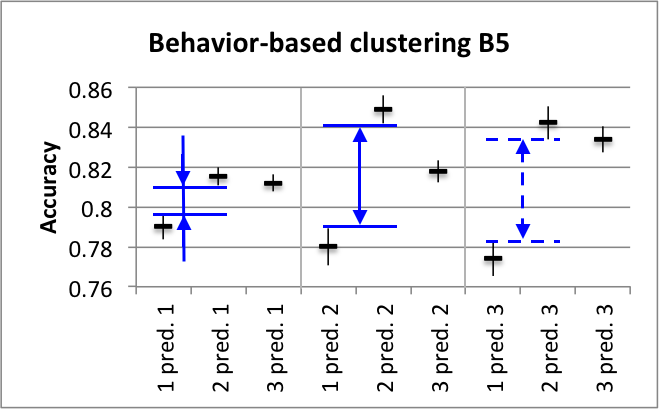
\includegraphics[width=0.7\columnwidth]{figures/behavior_clust_B5.png}
\caption{Between-cluster student group model prediction accuracy differences for Behavior-based clustering B5.}%\vspace{-15pt}
\label{fig:graph-clusters-B5}
\end{figure}

\section{A Deeper Analysis of Cluster Differences}

\subsection{What Differences Do Behavior-Based Clusters Show?}

Our findings from performance prediction with behavior-based clusters demonstrated that the discovered clusters (tinkerers, movers) were not performance-based stereotypes. In other words, the two clusters that we found did not differ by performance sufficiently enough to form stereotypes that could predict student's performance and serve as a basis for personalization. Whilst the clusters failed to separate students into classic performance-based stereotypes (weak, strong), we observed that they separated student into quite distinctive groups with stable but different behavior. Yet, given the belief of some programming instructors that tinkering is not a good problem solving behavior, we want to perform a deeper performance-focused analysis of our discovered pattern-based clusters. In this section, we inspect clusters' performance in more detail. 

\subsubsection{Tinkerers Are Less Efficient and Have Lower Grades}

To gain an insight into how the two behavior groups differed in terms of their performance, we looked int the a set of performance measures that includes: 1) number of problems that student attempted, 2)  number of problems that student solved, 3) average steps to solve the problem, where steps includes only test, run, and submit snapshots, 4) average time spent on solving the problem, 5) effectiveness score, and 6) course grade. Effectiveness score is a measure of instructional efficiency and represents student performance on the problems that student solved and the mental effort that student spent on solving those problems. Here, we chose time on problem-solving as an approximate measure of student mental effort and compute the effectiveness score as introduced in \cite{paas1993efficiency}. 

Table \ref{table:perfcompare} presents performance statistics for each of the aforementioned measures among students in cluster 1 (tinkerers), and students in cluster 2 (movers).  Wilcoxon ranked sum test was performed to measure the difference on each performance measure in cluster 1 and cluster. As it can be seen from the table, there is a significant difference between the two clusters in several cases. On average, students in cluster 2, made fewer steps to solve the problem ($M_2=3.4, M_1=5.9$), were faster in solving the problems ($M_2=630.0, M_1=998.1$), and as a result, were also more efficient in solving the problems ($M_2=0.4, M_1=-0.3$). Furthermore, average grade was also higher in cluster 2 than in cluster 1 ($M_2=3.4,M_1=2.9$). While all parameters known as signs of good performance point to cluster 2, we should be careful when interpreting this results as a clear sign of the cluster 2 problem-solving superiority. Making fewer larger steps is the very essence of problem solving approach of cluster 2, no surprise that students from this clusters looked more efficient. On the other hand, there was no significant difference between clusters in respect of the number of solved problems, although cluster 2 attempted more problems and solved more at average  compared to cluster 1.

\begin{table}[thb]
\centering
\begin{tabular}{@{}lccc@{}}
\small\textit{Performance Measure}  & \small\textit{Cluster 1} & \small\textit{Cluster 2} & \small\textit{Wilcoxon Test} \\
\midrule
\small\textit{\#Attmpted Probs.} & 81.3 ( 1.7) & 82.8 ( 1.3) & \num{73456} \\
\small\textit{\#Solved Probs.} & 68.1 ( 1.4) & 70.9 ( 1.0) & \num{68860} \\
%\small\textit{Solved Probs. (Ratio)} & 0.9 ( 0.0) & 0.9 ( 0.0) & \num{61371}$^{\ast\ast\ast}$ \\
\small\textit{Avg. Attempts to Solve} & 5.9 ( 0.2) & 3.4 ( 0.1) & \num{123790}$^{\ast\ast\ast}$\\
\small\textit{Avg. Time to Solve} & 998.1 (27.5) & 630.0 (16.7) & \num{111950}$^{\ast\ast\ast}$\\
\small\textit{Effectiveness Score} & -0.3 ( 0.1) & 0.4 ( 0.0) & \num{7253}$^{\ast}$\\
\small\textit{Course Grade} & 2.9 ( 0.2) & 3.4 ( 0.1) & \num{43068}$^{\ast\ast\ast}$ \\ \midrule
\multicolumn{4}{l}{\footnotesize $^{\ast}:p<.05$; \;\;\; $^{\ast\ast\ast}:p<.001$}
\end{tabular}
\caption{Performance statistics (Mean,SE) for students within Cluster 1 $(N=295)$, and students within Cluster 2 $(N=503)$. Wilcoxon Rank Sum was performed to compare performance of Clusters 1 and  2.}\vspace{-5pt}
\label{table:perfcompare}
\end{table}

\subsubsection{Patterns Show a Tendency Towards Low-High Performance}
From what we observed from clustering groupings, we know that one group was thinking in a constructive manner, that is students in cluster 2 who, often, thought for a long time, added concepts, and increased code correctness (see patterns \textit{{\_}AA}, \textit{AA}, \textit{AA{\_}} in Figure \ref{fig:clusters}). Students in cluster 1, on the other hand, seems to be weaker because, unlike cluster 2, they had more unsuccessful steps, they added concepts with no test being passed, or they changed (added/removed) concepts that did not influence the code correctness (see patterns \textit{Dd}, \textit{dD}, \textit{DE} in Figure \ref{fig:clusters}). Apparently, cluster 1 represents students who are less efficient in their problem-solving -- evaluated by performance measures like effectiveness score, and average attempts for solving the problem. So, it seems likely for weaker students to be in this group. 

When we looked further at the relationship between the micro-patterns in each group and the performance measures, we found that certain patterns are positively or negatively associated with performance\footnote{This analysis was performed by modeling performance measure of interest with the generalized linear model. Dependent variables were micro-patterns that had little correlation, if any.}. In particular, some patterns that represent mostly tinkering behavior turned out to be negatively related to both number of problems that student solved and their effectiveness score (\textit{{\_}jj}, \textit{JjJ}, \textit{ic{\_}}, \textit{{\_}JJJ}, \textit{jJJ}, \textit{JJk}, \textit{{\_}JK}, \textit{FF}). On the other hand, we found an instance of a constructive building pattern (\textit{{\_}AAD}) to be positively associated with both of these measures. Additionally, we observed that a pattern could have a different impact on different measures. In our case, pattern \textit{bA} was positively related to the number of solved problems and negatively related to effectiveness score.

\subsubsection{Both Groups Include a Mixture of Strong and Weak Students}

Why the tendency toward low- and high- performance among tinkerers and movers did not resulted in a grouping that reflects performance-based stereotypes? This is explained by elaborating on how weak and strong students were dispersed within the two groups. There were strong/weak students who exhibited similar problem-solving behavior. To check this hypothesis, we compared the overlap between the clustering that resulted in two groups of tinkerers and movers (i.e., clustering \textit{B4}) and the two performance-based clustering (i.e., \textit{Problem Solved}, and \textit{Percent Correct}). We found little overlap between groups that were found by these clustering approaches (See Table \ref{table:behavior-groups}, rows 4-5 in column \textit{B4}, the overlap is less than 0.30). This is sufficiently strong evidence to let us conclude that there were both weak and strong students among movers and tinkerers. 

So, it appeared that strong and weak students were dispersed within each behavior group. We observed that a large chunk of students in cluster 1 (tinkerers) were strong students. These students performed well, but they had the same problem-solving behavior as poor students. This clarifies that behavior-based clusters represented different behaviors in solving problems and not the classic weak/strong performance groups. %These behavior-based groups could not be interpreted as performance-based stereotypes, yet, they could associate an overall tendency in performance for students who are within those groups. 

\section{Discussion and Future Work}
%%%%%%%

\subsection{There Are Not Even Two Different Student Stereotypes}

We have set out to find at least two groups of students, not necessarily representing 100\% of student sample available to us, but different enough so that we could reliably say they learn differently and could benefit from different kinds of adaptation, different computer-aided help system setups, or different methods of instruction, if it comes to that.

Just like authors of \cite{yudelson2014bdbbd} in the domain of K-12 math, we found that there is always one sub-sample of students that can effectively be used to build a model of student learning for the whole population available. While this is a null result (better yet a repeated one), it is an important one. This means that there are likely no stereotypes like ``good students'' or ``bad students''. There are likely no ``fast learners'' or ``slow learners''. There are students who approach learning differently and the distinction between these approaches are orthogonal to the conventional dimensions we apply to quantify learning.


\subsection{How Should Our Findings Be Interpreted}

Mining behavior of students in problem-solving activities helped us find individual differences in how student solved programming problems. Some students preferred to think for a long time, and added the concepts that increased the correctness at the first try, while some students tended to take more tinkering steps by adding, removing, or changing the existing concepts in the program code that did not result in the immediate increase of  code correctness.  Indeed, for some students exhibiting the latter problem-solving behavior might be a sign of poor performance, but we should have this in mind that there are also students who have same behavior but are doing very well regarding their performance. This is an important finding, particularly for MOOCs design, as it points out that we should not necessarily intervene when students exhibit more tinkering steps. This is the way some students solve problems, and they can do well with that.

A set of simpler and behavior-bases grouping approaches we tried did not result in discernible differences in cross-prediction accuracies. Namely, there is always one sub-population of students that contributes a model that could be universally used for all. This means that grouping students for targeted adaptation is not likely to be useful. Students, whether classified by their demographics, overall performance, or approach to solving programming problems, should not be treated as stereotypes, but rather considered in the context of a larger or smaller topic of the material, or even on the finer-grained level of a problem-solving session.


\subsection{Potential Limitations}

We used traditional programming course and programming MOOC course data that come from the University in Europe. The system of education in that country might be different from rest of the World. It is likely that the sample of students we have obtained could have influenced the behavior grouping and the performance of the models of learning. In future work, we would like to get a larger more representative sample of student data and rerun our analysis to validate and, possibly, reconfirm our findings. Also, we plan to reduce the program concepts that we used in the modeling to only crucial ones. This would reduce inaccuracies  that were due to noise in data.

%%%%%

% BALANCE COLUMNS
%\balance{}

% REFERENCES FORMAT
% References must be the same font size as other body text.
%\bibliographystyle{SIGCHI-Reference-Format}
%\bibliography{ref}
\bibliographystyle{abbrv}
\bibliography{ref}

\end{document}

%%% Local Variables:
%%% mode: latex
%%% TeX-master: t
%%% End:
